
\documentclass[aspectratio=169]{beamer}
%\usetheme{Boadilla}
\usetheme{Warsaw}


\usepackage{listings}
\usepackage{xcolor}
 
\definecolor{codegreen}{rgb}{0,0.6,0}
\definecolor{codegray}{rgb}{0.5,0.5,0.5}
\definecolor{codepurple}{rgb}{0.58,0,0.82}
\definecolor{backcolour}{rgb}{0.95,0.95,0.92}
 
\lstdefinestyle{mystyle}{
    language=Python,
    backgroundcolor=\color{backcolour},   
    commentstyle=\color{codegreen},
    keywordstyle=\color{magenta},
    numberstyle=\tiny\color{codegray},
    stringstyle=\color{codepurple},
    basicstyle=\ttfamily\tiny,
    breakatwhitespace=false,         
    breaklines=true,                 
    captionpos=b,                    
    keepspaces=true,                 
    numbers=left,                    
    numbersep=5pt,                  
    showspaces=false,                
    showstringspaces=false,
    showtabs=false,                  
    tabsize=2
}


 
\lstset{style=mystyle}
%\usepackage{minted}


\usepackage{datetime}
\newdateformat{specialdate}{\twodigit{\THEDAY}-\twodigit{\THEMONTH}-\THEYEAR}
\date{\specialdate\today}


%\renewrobustcmd{\mkbibfootnote}{\normalsize\footnotemark\footnotetext}
\setbeamerfont{footnote}{size=\tiny}

\setbeamertemplate{footline}[frame number]{} % Evita que \pause 
\setbeamertemplate{bibliography item}{\insertbiblabel} % Numeros en las referenicas en vez de iconos




%%%%%%%%%%%%%%%%%%%%%%%%%%%%%%%%%%%%%%%%%%%%%%%%%%%%%%%%%%%%%%%%%%%%%%%%%%%%%
% HEADER
%%%%%%%%%%%%%%%%%%%%%%%%%%%%%%%%%%%%%%%%%%%%%%%%%%%%%%%%%%%%%%%%%%%%%%%%%%%%%

%\title[\arabic{page} ]{Advanced Computer Graphics}
\title[Arrays]{SEARCHING AND SORTING ALGORITHMS}
% Sin subtitulos
\subtitle{6.0001 LECTURE 12}
\author{Kevin Alejandro Hernandez Campillo}
\institute[UPV]{Polytechnic University of Victoria}
\date[]{September-December 2022}
\logo{\pgfimage[width=1cm,height=1cm]{graphics/logo_upv_transparente}}			% Logo on all slides (pdf,png,jpg,eps)
\titlegraphic{
\includegraphics[height=1.5cm]{graphics/logo_upv_transparente} \hfil 
\includegraphics[height=1.5cm]{graphics/python.png}}	% Logo on title slide


\usepackage{etoolbox}
\makeatletter
\patchcmd{\@verbatim}
  {\verbatim@font}
  {\verbatim@font\tiny}
  {}{}
\makeatother


\begin{document}

% Diapositiva de título
\begin{frame}[plain]
  \titlepage
\end{frame}

\begin{frame}[fragile]{SEARCH ALGORITHMS}

\begin{itemize}
\item search algorithm – method for finding an item or group of items with specific properties within a collection of items

\item collection could be implicit
\begin{itemize}
\item example – find square root as a search problem
\begin{itemize}
\item exhaustive enumeration
\item bisection serch
\item Newton-Raphson
\end{itemize}
\end{itemize}
\item collection could be explicit
\begin{itemize}
\item example - is a stident record in a stored collection of data?
\end{itemize}

\end{itemize}
\end{frame}

\begin{frame}[fragile]{SERCHING ALGORITHMS}
\begin{itemize}
\item linear search
\begin{itemize}
\item  \textcolor{red}{brute force} search (aka British Museum algorithm)
\item list does not have to be sorted
\end{itemize}
\item bisection search
\begin{itemize}
\item list \textcolor{red}{MUST be sorted} to give correct answer
\item saw two different implementations of the algorithm
\end{itemize}
\end{itemize}
\end{frame}


\begin{frame}[fragile]{LINEAR SERCH ON \textcolor{red}{UNSORTED} LIST:RECAP}
\begin{lstlisting}
	def linear_serch(L,e):
		found = False
		for i in range(len(L)):
			if e==L[i]:
				found = True
		return found    
\end{lstlisting}
 
\begin{itemize}
\item must look through all elements to decide it’s not there
\item O(len(L)) for the loop*O(1) to test if e == L[i]
\item overall complexity is O(n)-where n is len(L). Assumes we can retrieve element of list in constant time
\item speed up a little by returning True here, but speed up doesn't impact worst case
\begin{lstlisting}
if e==L[i]:
	found = True
\end{lstlisting} 
\end{itemize}
\end{frame}

\begin{frame}[fragile]{LINEAR SERCH ON \textcolor{red}{UNSORTED} LIST:RECAP}
\begin{columns}
\column{0.55\linewidth}
Example code:
\begin{lstlisting}
def linear_serch(L,e):
		found = False
		for i in range(len(L)):
			if e==L[i]:
				found = True
		return found
lista = [4,2,6,7]
print(linear_serch(lista,8))
print(linear_serch(lista,6))
\end{lstlisting}
\column{0.40\linewidth}
Output:
\begin{block}{}
\begin{verbatim}
False
True
\end{verbatim}
\end{block}
\end{columns}
\end{frame}


\begin{frame}[fragile]{LINEAR SERCH ON \textcolor{red}{SORTED} LIST:RECAP}
\begin{lstlisting}
def search(L,e):
	for i in range(len(L)):
		return True
	if L[i] > e:
		return False
	return False
\end{lstlisting}
\begin{itemize}
\item musto only look until reach a number geater than e
\item O(len(L)) for the loop*O(1) to test if e==L[i]
\item overall complexity is \textcolor{red}{O(n)-where n is len(L)}
\end{itemize}
\end{frame}

\begin{frame}[fragile]{LINEAR SERCH ON \textcolor{red}{SORTED} LIST:RECAP}
\begin{columns}
\column{0.55\linewidth}
Example code:
\begin{lstlisting}
def search(L,e):
	for i in range(len(L)):
		return True
	if L[i] > e:
		return False
	return False
lista = [3,4,6,8,9]
print(linear_serch(lista,6))
print(linear_serch(lista,5))
\end{lstlisting}
\column{0.40\linewidth}
Output:
\begin{block}{}
\begin{verbatim}
True
False
\end{verbatim}
\end{block}
\end{columns}
\end{frame}

\begin{frame}{USE BISECTION SERCH: RECAP}
\begin{enumerate}
\item Pick an index, i, that divides list in half
\item Ask if L[i]==e
\item if not, ask if L[i] is larger or smaller than e
\item Depending on answare, sherch left or right half of L for e
\end{enumerate}

A new version of a divide-and conqer algorithm
\begin{itemize}
\item Breake into smaller version of problema(smaller list), puls some simple operations
\item Answare to smaller version is answer to original problem
\end{itemize}
\end{frame}

\begin{frame}{BISECTION SERCH IMPLEMENTATION: RECAP}
\lstinputlisting{bisect_serch2.py}
\end{frame}


\begin{frame}{COMPLEXITY OF BISECTION SEARCH: RECAP}
\begin{itemize}
\item \textcolor{red}{\textbf{bisect\_serch2}} and its helper
\begin{itemize}
\item O(log n) bisection serch calls
\begin{itemize}
\item reduce size of problem by factor of 2 on each step
\end{itemize}
\item pass list and indices as parameters
\item list never copied, just re-passed as pointer
\item constant work inside funcion
\item $\rightarrow$ \textcolor{red}{\textbf{O(log n)}}
\end{itemize}

\end{itemize}

\end{frame}

\begin{frame}[fragile]{BISECTION SERCH IMPLEMENTATION: RECAP}
\begin{columns}
\column{0.65\linewidth}
Example code:
\lstinputlisting{bisect_serch2_ex.py}
\column{0.30\linewidth}
Output:
\begin{block}{}
\begin{verbatim}
True
False
\end{verbatim}
\end{block}
\end{columns}

\end{frame}


\begin{frame}{SEARCHING A SORTED LIST --n is len(L)}
\begin{itemize}
\item using \textcolor{red}{\textbf{linear search}}, search for an element is \textcolor{red}{\textbf{O(n)}}
\item using \textcolor{red}{\textbf{binary search}}, can search for an element in \textcolor{red}{\textbf{O(log n)}}
\begin{itemize}
\item assumes the \textcolor{red}{\textbf{list is sorted!}}
\end{itemize}

\item when does it make sense to \textcolor{red}{\textbf{sort first then search}}?
\begin{itemize}
\item  SORT + O(log n) $<$ O(n) $\rightarrow$ SORT $<$ O(n) - O(log n)
\item when sorAng is less than O(n)
\end{itemize}
\item \textcolor{red}{NEVER TRUE!}
\begin{itemize}
\item to sort a collecEon of n elements must look at each one at
least once!
\end{itemize}
\end{itemize}
\end{frame}

\begin{frame}{AMORTIZED COST --n is len(L)}
\begin{itemize}
\item why bother sorting first?
\item in some cases, may \textcolor{red}{\textbf{sort a list once}} then do \textcolor{red}{\textbf{many searches}}
\item \textcolor{red}{\textbf{AMORTIZE cost}} of the sort over many searches
\item SORT + k\*O(log n) $<$ k\*O(n) \\
	$\rightarrow$ for large K, \textcolor{red}{\textbf{SORT time becomes irrelevant,}} if cost of sorting is small enough
\end{itemize}
\end{frame}

\begin{frame}{SORT ALGORITHMS}
\begin{itemize}
\item  Want to efficiently sort a list of entries (typically
numbers)
\item Will see a range of methods, including one that is
quite efficient
\end{itemize}
\end{frame}

\begin{frame}{MONKEY SORT}
\begin{columns}
\column{0.55\linewidth}
\begin{itemize}
\item aka bogosort, stupid sort, slowsort, permutaAon sort, shotgun sort
\item  to sort a deck of cards
\begin{itemize}
\item throw them in the air
\item pick them up
\item are they sorted?
\item repeat if not sorted
\end{itemize}

\end{itemize}
\column{0.40\linewidth}
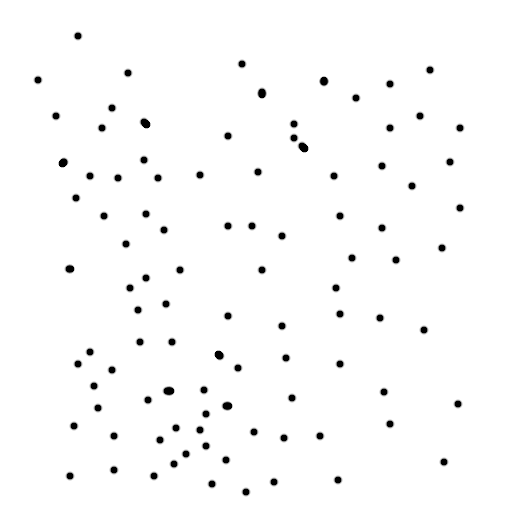
\includegraphics[scale=1]{graphics/monkey_sort.png}
\end{columns}
\end{frame}

\begin{frame}[fragile]{COMPLEXITY OF BOGO SORT}
\begin{lstlisting}
def bogo_sort(L):
	while not is_sorted(L):
		random.shuffle(L)
\end{lstlisting}
\begin{itemize}
\item best case: \textcolor{red}{\textbf{O(n) where n is len(L)}} to check if sorted
\item worst case: O(?) it is \textcolor{red}{\textbf{unbounded}} if really unlucky

\end{itemize}
\end{frame}

\begin{frame}[fragile]{COMPLEXITY OF BOGO SORT}
\begin{columns}
\column{0.65\linewidth}
Example code:
\lstinputlisting{bogo_sort_ex.py}
\column{0.30\linewidth}
Output:
\begin{block}{}
\begin{verbatim}
[1, 2, 7, 9, 10]
\end{verbatim}
\end{block}
\end{columns}

\end{frame}

\begin{frame}{BUBBLE SORT}
\begin{columns}
\column{0.45\linewidth}
\begin{itemize}
\item \textcolor{red}{\textbf{compare consecutive pairs}} of elements
\item \textcolor{red}{\textbf{swap elements}} in pair such that smaller is first
\item when reach end of list,\textcolor{red}{\textbf{start over}} again
\item stop when \textcolor{red}{\textbf{no more swaps}} have been made
\item largest unsorted element always at end a\_er pass, so at most n passes
\end{itemize}
\column{0.45\linewidth}
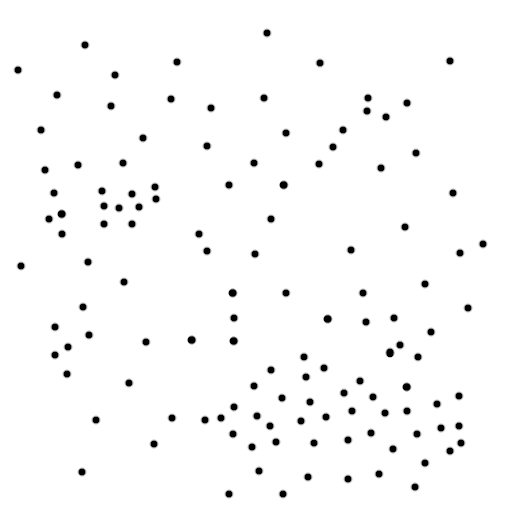
\includegraphics[scale=1]{graphics/bubble_sort.png}
\end{columns}
\end{frame}

\begin{frame}[fragile]{COMPLEXITY OF BUBBLE SORT}
\begin{lstlisting}
def bubble_sort(L):
	swap = False
	while not swap:
		swap = True
		for j in range(1,len(L)):
			if L[j-1] > L[j]:
				swap = False
				temp = L[j]
				L[j] = L[j-1]
				L[j-1] = temp
\end{lstlisting}
\begin{itemize}
\item inner for loop is for doing the \textcolor{red}{\textbf{comparisons}}
\item outer while loop is for doing \textcolor{red}{\textbf{multiple passes}} unti no more swaps
\item \textcolor{red}{\textbf{O($n^2$) where n is len(L)}} to do len(L)\-1 comparsions and len(L)\-1 passes
\end{itemize}
\end{frame}

\begin{frame}[fragile]{COMPLEXITY OF BUBBLE SORT}
\begin{columns}
\column{0.65\linewidth}
Example code:
\begin{lstlisting}
def bubble_sort(L):
    swap = False
    while not swap:
        swap = True
        for j in range(1,len(L)):
            if L[j-1] > L[j]:
                swap = False
                temp = L[j]
                L[j] = L[j-1]
                L[j-1] = temp
    return L    
lista=[7,1,4,5,3]
print(bubble_sort(lista))
\end{lstlisting}
\column{0.30\linewidth}
Output:
\begin{block}{}
\begin{verbatim}
[1, 3, 4, 5, 7]
\end{verbatim}
\end{block}
\end{columns}
\end{frame}

\begin{frame}{SELECTION SORT}
\begin{itemize}
\item first step
\begin{itemize}
\item extract \textcolor{red}{\textbf{minimum element}}
\item \textcolor{red}{\textbf{swap it}} with element at \textcolor{red}{\textbf{index 0}}
\end{itemize}
\item subsequent step
\begin{itemize}
\item in remaining sublist, extract \textcolor{red}{\textbf{minimum element}}
\item \textcolor{red}{\textbf{swap it}} with the element at \textcolor{red}{\textbf{index 1}}
\end{itemize}
\item keep the left portion of the list sorted
\begin{itemize}
\item at i'step, \textcolor{red}{\textbf{first i elements in list are sorted}}
\item all other elements are bigger than first i elements
\end{itemize}
\end{itemize}
\end{frame}


\begin{frame}{ANALYZING SELECTION SORT}
\begin{itemize}
\item loop invariant
\begin{itemize}
\item given prefix of list L[0:i] and suffix L[i+1:len(L)], then prefix is sorted and no element in prefix is larger than smallest element in suffix
\begin{enumerate}
\item  base case: prefix empty, suffix whole list - invariant true
\item  induction step: move minimum element from suffix to end of prefix. Since invariant true before move, prefix sorted after append
\item when exit, prefix is entire list, suffix empty, so sorted
\end{enumerate}
\end{itemize}
\end{itemize}
\end{frame}

\begin{frame}[fragile]{COMPLEXITY OF SELECTION SORT}
\begin{lstlisting}
def selection_sort(L):
	suffixSt = 0
	while suffixSt != len(L):
		for i in range(suffixSt, len(L)):
			if L[i]<L[suffixSt]:
				L[suffixSt], L[i] = L[i], L[suffixSt]
		suffixSt +=1
\end{lstlisting}

\begin{itemize}
\item outer loop executes len(L) times
\item inner loop executes len(L) – i tomes
\item complexity of selection sort is \textcolor{red}{\textbf{O($n2$) where n is len(L)}}
\end{itemize}
\end{frame}

\begin{frame}[fragile]{COMPLEXITY OF SELECTION SORT}
\begin{columns}
\column{0.65\linewidth}
Example code:
\begin{lstlisting}
def selection_sort(L):
    suffixSt = 0
    while suffixSt != len(L):
        for i in range(suffixSt, len(L)):
            if L[i]<L[suffixSt]:
                L[suffixSt], L[i] = L[i], L[suffixSt]
        suffixSt +=1
    return L
lista=[4,2,5,9,3]
print(selection_sort(lista))
\end{lstlisting}
\column{0.30\linewidth}
Output:
\begin{block}{}
\begin{verbatim}
[2, 3, 4, 5, 9]
\end{verbatim}
\end{block}
\end{columns}
\end{frame}

\begin{frame}{MERGE SORT}
\begin{itemize}
\item use a divide-and-conquer approach:
\begin{enumerate}
\item if list is of length 0 or 1, already sorted
\item if list has more than one element, split into two lists, and sort each
\item merge sorted sublists
\begin{enumerate}
\item look at first element of each, move smaller to end of the result
\item when one list empty, just copy rest of other list
\end{enumerate}
\end{enumerate}
\end{itemize}
\end{frame}

\begin{frame}{MERGE SORT}
\begin{itemize}
\item divide and conquer
\end{itemize}
\begin{center}
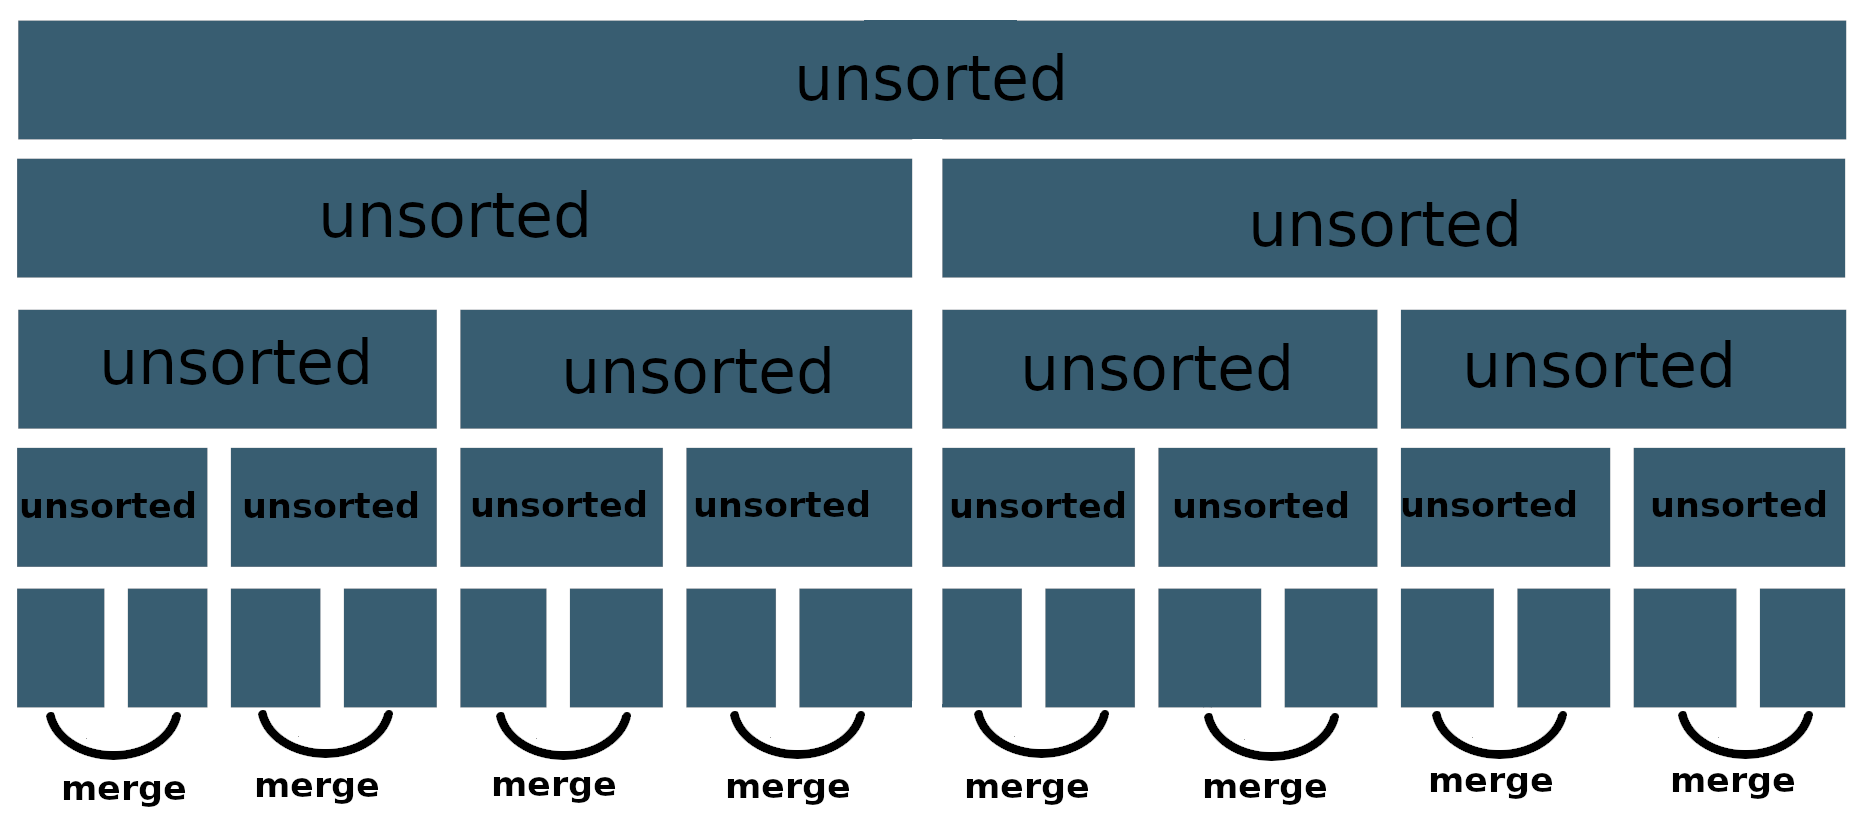
\includegraphics[scale=0.70]{graphics/marge_sort.png}
\end{center}
\begin{itemize}
\item \textcolor{red}{\textbf{split list in half}} until have sublists of only 1 element

\end{itemize}

\end{frame}

\begin{frame}{MERGE SORT}
\begin{itemize}
\item divide and conquer
\end{itemize}
\begin{center}
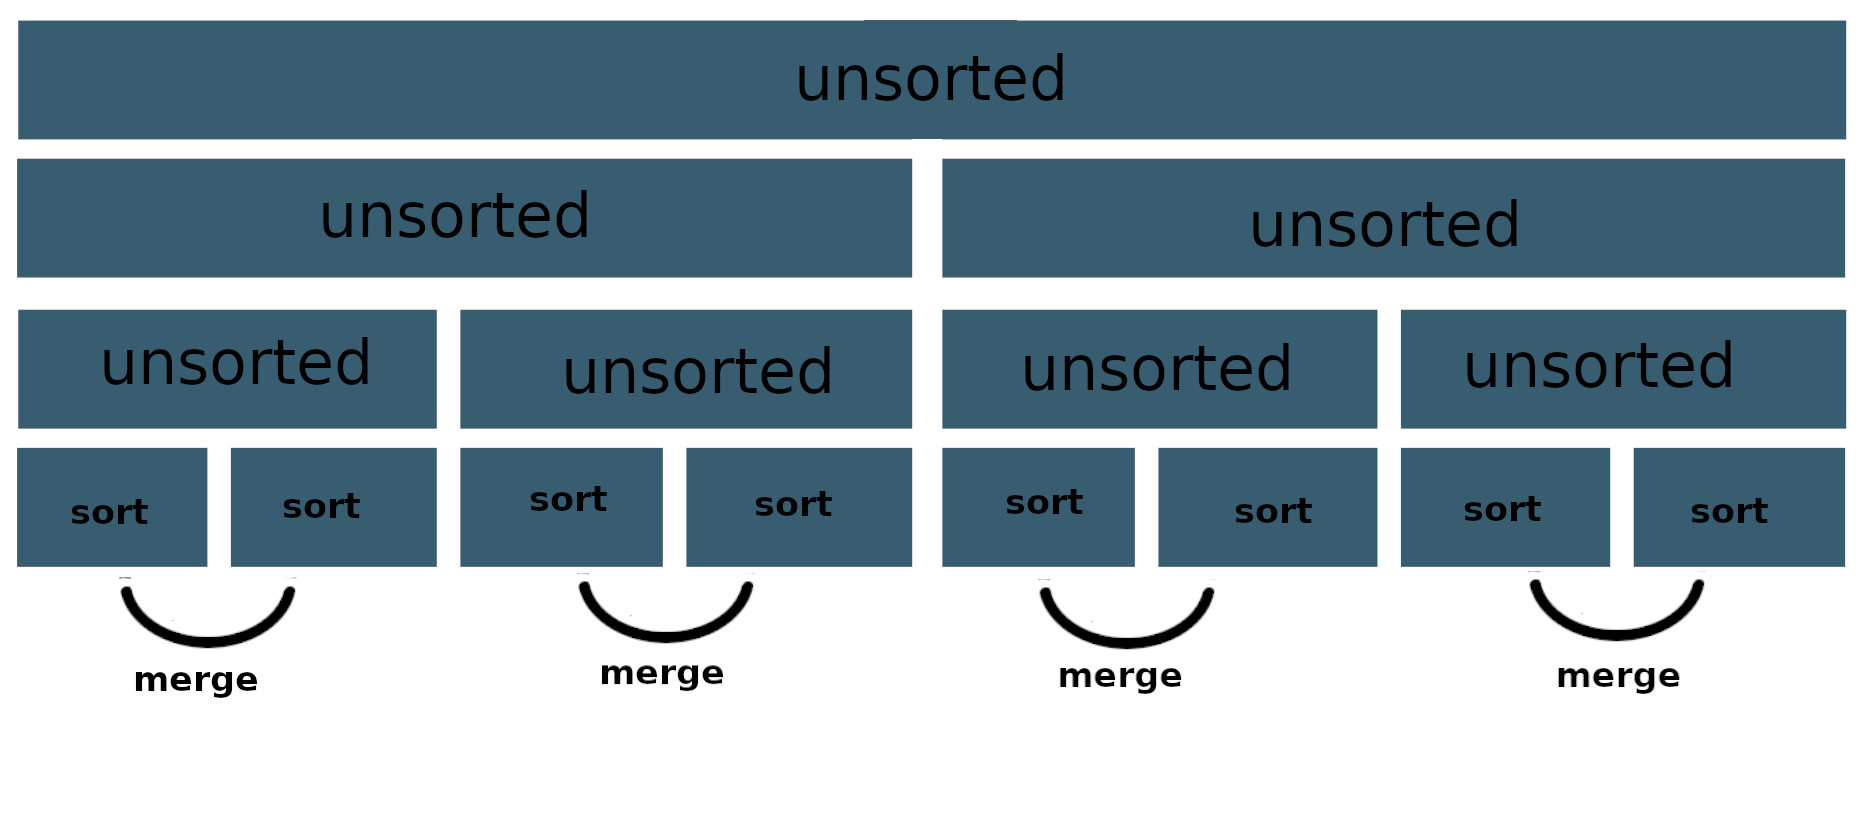
\includegraphics[scale=0.70]{graphics/marge_sort2.png}
\end{center}
\begin{itemize}
\item merge such that \textcolor{red}{\textbf{sublists will be sorted after merge}}
\end{itemize}
\end{frame}

\begin{frame}{MERGE SORT}
\begin{itemize}
\item divide and conquer
\end{itemize}
\begin{center}
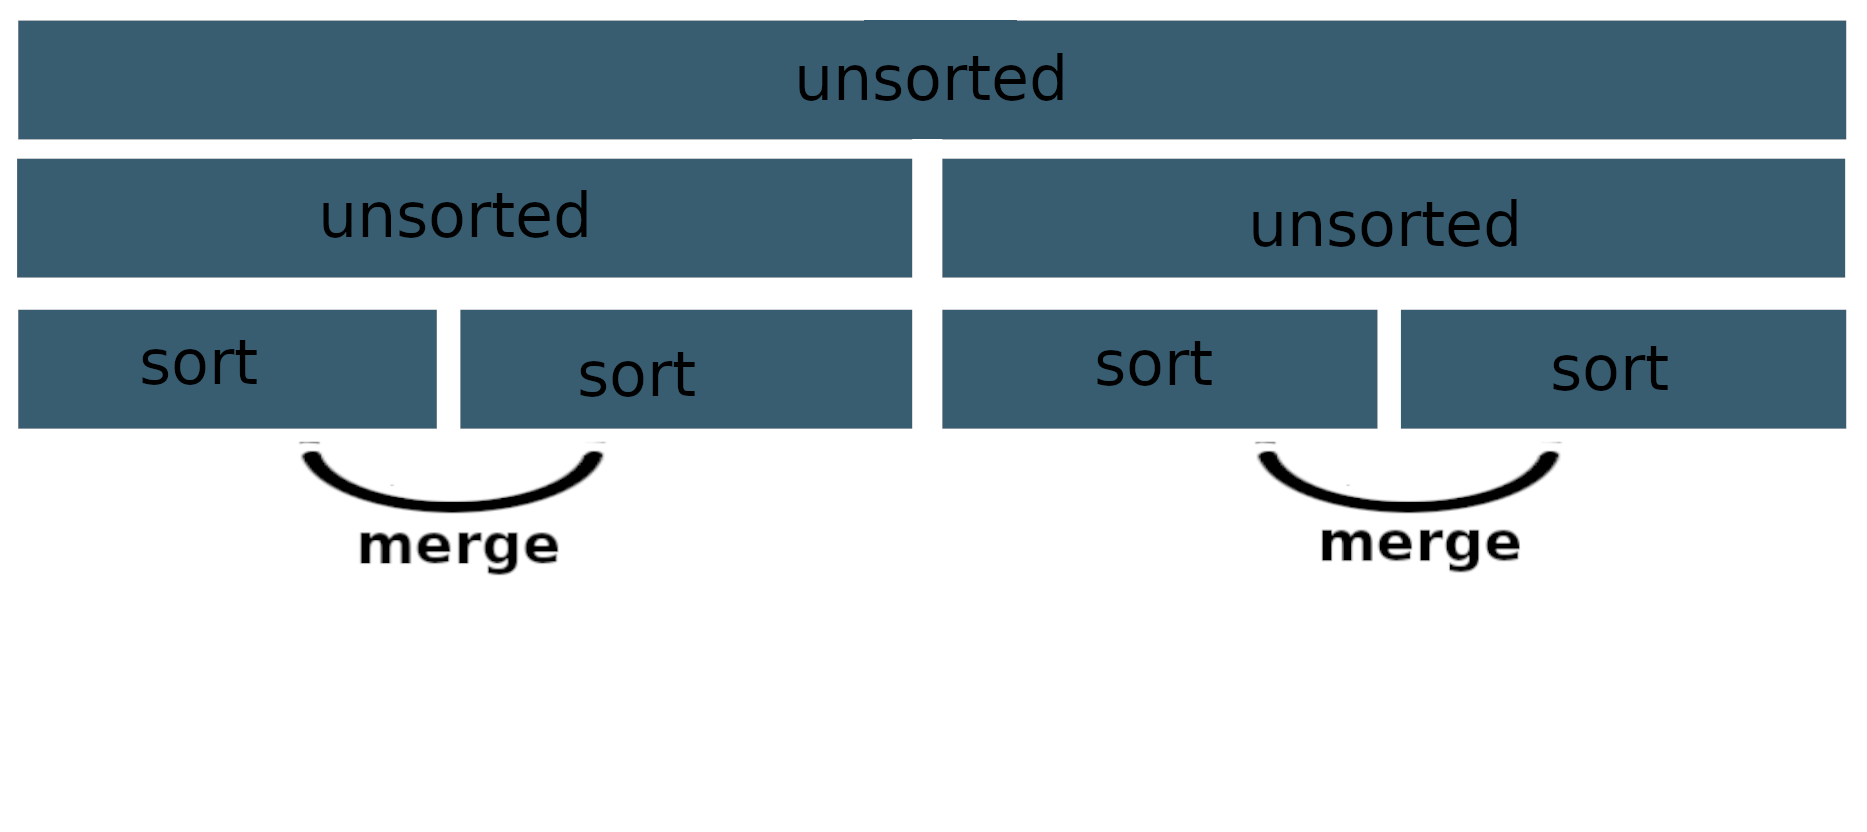
\includegraphics[scale=0.70]{graphics/marge_sort3.png}
\end{center}
\begin{itemize}
\item merge sorted sublists
\item sublists will bee sorted after merge
\end{itemize}
\end{frame}

\begin{frame}{MERGE SORT}
\begin{itemize}
\item divide and conquer
\end{itemize}
\begin{center}
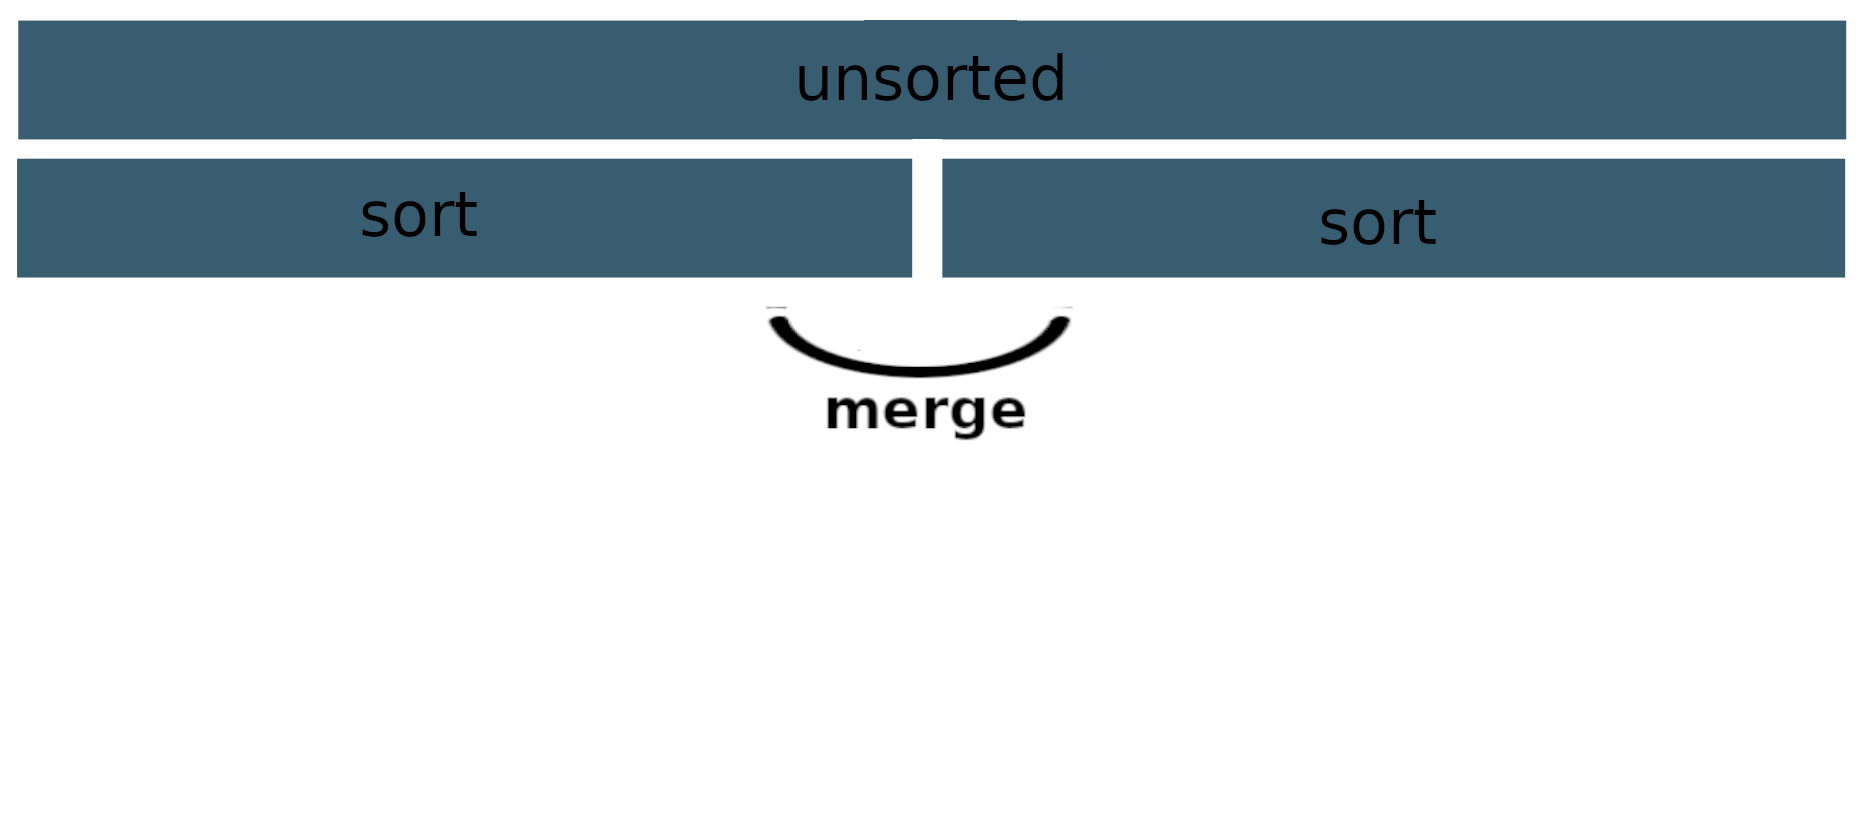
\includegraphics[scale=0.70]{graphics/marge_sort4.png}
\end{center}
\begin{itemize}
\item merge sorted sublists
\item soblists will be sorted after merge
\end{itemize}
\end{frame}

\begin{frame}{MERGE SORT}
\begin{itemize}
\item divide and conquer - done!
\end{itemize}
\begin{center}

\includegraphics[scale=0.70]{graphics/marge_sort5.png}
\end{center}
\end{frame}

\begin{frame}{EXAMPLE OF MERGING}
\begin{columns}
\column{0.24\linewidth}
Left in list 1\par
[1,5,12,18,19,20]\par
[5,12,18,19,20]\par
[5,12,18,19,20]\par
[5,12,18,19,20]\par
[5,12,18,19,20]\par
[12,18,19,20]\par
[18,19,20]\par
[18,19,20]\par
[]
\column{0.24\linewidth}
Left in list 2\par
[2,3,4,17]\par
[2,3,4,17]\par
[3,4,17]\par
[4,17]\par
[17]\par
[17]\par
[17]\par
[]\par
[]
\column{0.2\linewidth}
Compare\par
1,2\par
5,2\par
5,3\par
5,4\par
5,17\par
12,17\par
18,17\par
18,--
\column{0.28\linewidth}
Result\par
[]\par
[1]\par
[1,2]\par
[1,2,3]\par
[1,2,3,4]\par
[1,2,3,4,5]\par
[1,2,3,4,5,12]\par
[1,2,3,4,5,12,17]\par
[1,2,3,4,5,12,17,18,19,20]
\end{columns}
\end{frame}

\begin{frame}[fragile]{MERGING SUBLISTS STEP}
\begin{lstlisting}
def merge(left, right):
	result = []
	i,j = 0,0
	while i < len(left) and j < len(right):
		if left[i] < right[j]:
			result.append(left[i])
			i += 1
		else:
			result.append(right[j])
			j += 1
	while (i < len(left)):
		result.append(left[i])
		i += 1
	while (j < len(right)):
		result.append(right[j])
		j += 1
	return result

\end{lstlisting}

\end{frame}


\begin{frame}[fragile]{MERGING SUBLISTS STEP - CODE EXPLAINED}
\begin{lstlisting}
if left[i] < right[j]:
	result.append(left[i])
	i += 1
else:
	result.append(right[j])
	j += 1
\end{lstlisting}
\begin{itemize}
\item left and right sublists are ordered
\item move indices for sublists depending on which sublist holds next smallest element
\end{itemize}
\begin{lstlisting}
while (i < len(left)):
		result.append(left[i])
		i += 1
\end{lstlisting}
\begin{itemize}
\item when right sublist is empty
\end{itemize}

\begin{lstlisting}
while (j < len(right)):
		result.append(right[j])
		j += 1
\end{lstlisting}
\begin{itemize}
\item when left sublist is empty
\end{itemize}
\end{frame}

% Nota1: La siguiente diapositiva muestra ejemplos de como insertar pequeños pedazos de codigo (declaracion de variables, codigos de no mas de 10 lineas) sin requerir guardar el codigo en un archivo por separado. Uselo 
% NOta2: Siempre que quieran poner codigo a mano y no proveniente de un archivo, deben establecer el parametro fragile en este Frame
\begin{frame}[fragile]
\frametitle{Placing code in multiple columns}
When required, you should adjust the code to multiple columns as shown in this slide
\begin{columns}
\column{0.48\linewidth}
A variable is declared and represents a value that is expected to change throughout a program.
\begin{lstlisting}
age = 25
string = 'Cadena'  
\end{lstlisting}

An immutable variable is declared with the val keyword and represents a value that must remain constant throughout a program.
\begin{lstlisting}
goldenRatio = 1.618
\end{lstlisting}

\column{0.48\linewidth}

When a data type is not specified in a variable declaration, the variable’s data type can be inferred through type inference.
\begin{lstlisting}
color = "Purple" 
\end{lstlisting}


String concatenation is the process of combining Strings using the + operator.

\begin{lstlisting}
x = "Python is "
y = "awesome"
z =  x + y
print(z)
\end{lstlisting}
\end{columns}
\end{frame}

\begin{frame}[fragile]
\frametitle{Using Images in Beamer}
Images can be placed in one single column or in two (as shown in this slide)
\begin{columns}

\column{0.48\linewidth}
\begin{itemize}
\item Mobile Programming 
\item Intelligent Systems
\item Automaton and Languages
\end{itemize}
\column{0.48\linewidth}
\begin{center}

\includegraphics[width=0.98\linewidth]{graphics/Opengl-logo.png}    
\end{center}


\end{columns}
\end{frame}


\end{document}

